\documentclass[11pt]{article}

\usepackage[utf8]{inputenc}
\usepackage[T1]{fontenc}

\usepackage{amssymb}
\usepackage{amsthm}
\usepackage{amsmath}
\usepackage{mathtools}
\usepackage{mathabx}
%\usepackage{framed}
\usepackage{booktabs}
\usepackage{hyperref}
\usepackage{txfonts}
\usepackage{siunitx}



\hypersetup
	{ 
		colorlinks=true,       % false: boxed links; true: colored links
%		hidelinks,
		linkcolor=blue,          % color of internal links (change box color with linkbordercolor)
		citecolor=green,        % color of links to bibliography
		filecolor=magenta,      % color of file links
		urlcolor=cyan,           % color of external links
		linkbordercolor	= {1 0 0},
		citebordercolor	= {0 1 0},	
		urlbordercolor	= {0 1 1}
	}


%\usepackage{fontspec}
%\setmainfont{Clear Sans}
%\newfontfamily{\clearsans}{Clear Sans}

\newcommand{\definition}{\\ \textbf{Definition:} \hspace{1cm} }

\newcommand*{\QEDA}{\hfill\ensuremath{\blacksquare}}%
\newcommand*{\QEDB}{\hfill\ensuremath{\square}}%


\begin{document}
	\title{Kapitel 14 - Statische elektrische Felder}
		\author
		{Johannes Bilk
			\\
			{\small 	\texttt{me@talachem.de}}
		}
		\date{\today}
	\maketitle
	\tableofcontents
	\setcounter{section}{13} %Hier f\"{a}ngt die Nummerierung an.
	
	\newpage
	
\section{Statische Elektrische Felder}	
	\subsection{ Elektrische Ladungen }	
	
	$\rightarrow$ Ab dem 17. Jahrhundert: Ursache für "elektrische Ph\"{a}nomene"; "neuartiger Stoff", elektrische Ladung\\
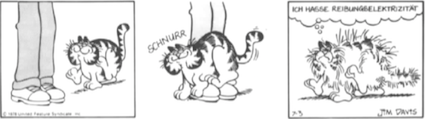
\includegraphics{skizzen/14/14_1B0}
		\subsubsection{ Reibungselektriziz\"{a}t }
		
			\begin{itemize}
			\item Zwei Arten von "elektrischen Zust\"{a}nden" sind erzeugbar:
				\begin{itemize}
				\item Gleichartige Zust\"{a}nde $\implies$ Abstoßung
				\item Ungleichartige Zust\"{a}nde $\implies$ Anziehung
			\end{itemize}
			\item Carles Du Fay (1730): positiv/negativ elektrische Ladung
			\item Benjamin Franklin (1750): Über-/Unterschuss an "elektrischen Fluiden"
			\item Lichtenberg (1778): Zuordnung der Polari\"{a}t
			\end{itemize}
			
			\fbox{\begin{minipage}{19em}
			Hargummi stab: reiben mit Pelz, Wolle: -\\
			Glas, Plexiglas: reiben mit Seide: +
			\end{minipage}}
			\linebreak\\
			Reibezeug: entgegengesetzte Polarit\"{a}t
			$\implies$ Ladungstrennung, nicht etwa Ladungserzeugung.
			\linebreak\\
			\subparagraph {Grunds\"{a}tzliches Messprinzip: Elektroskop:} \hfill \\
			
			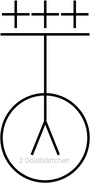
\includegraphics{skizzen/14/14_1B1}
			
			$\rightarrow$ Elektrometer $\rightarrow$ quantitative Messung
			\begin{itemize}
				\item "L\"{o}ffeln"; d.h. portionsweise Übertragung von Ladungen ist mglich
				\item Elektropendel: $\implies$ periodisches Umladen eines "Kugelpendel"
			\end{itemize}
			
			\subsubsection{Ladung ist eine skalare Gr\"{o}\ss{}e } Einheit 1C = 1 Coulomb, SI
				\begin{itemize}
					\item Zu jedem geladenen Elementarteilchen gibt es ein Elementarteilchen mit entgegengesetzter Ladung ($\rightarrow$ Ladungssymmetrie)
					\item Die Gesamtladung eines abgeschlossenen Systems bleibt erhalten ($\rightarrow$ Ladungserhaltung)
					\item Beispiel: Produktion eines $ e^+e^- $-Paares; $ E_\gamma \geq $ 1,02 MeV
				\end{itemize}
				
				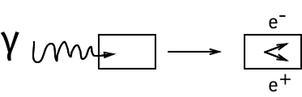
\includegraphics{skizzen/14/14_1B2}
				
				\newpage
				
				\noindent Nachweis: Blasenkammer im Magnetfeld:  \hfill \\
				Umkehrung: "Zerstrahlung" von Positronen; $E=m\cdot c^2$
				\begin{itemize}
					\item Ladungtr\"{a}ger haben stets eine Masse
					\item Ladung kann nicht (im Gegensatz zur Masse) in Energie umgewandelt werden, bleibt auch bei Zerfallsprozessen erhalten.
					\item Quantisierung der Ladung: Alle in der Natur vorkommenden Ladungen sind ganzzahlige Vielfache der Elementarladung: $e_0:=1,602\cdot10^{-19}C; 1C=1AS$
				\end{itemize}
				\subparagraph{Beispiele von Ladungen}
				\begin{itemize}
					\item Neutral: $\gamma, \nu, n$
					\item einfach geladen: $e^-,e^+,p, \bar{p}$
					\item zweifach geladen:: $He_2(2^+,Z:2)$
				\end{itemize}	
				

\subsubsection{ Quarks }	
\paragraph{Seit 60er Jahre}
Nukleonen bestehen aus Quarks, diese haben "drittelzahlige Ladungen"

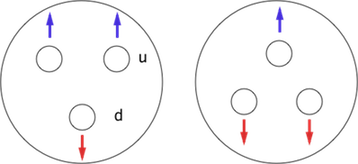
\includegraphics{skizzen/14/14_1B5}
\\
Up-Quarks:$u:+\frac{2}{3	}e_0$
\\
Down-Quarks:$d:-\frac{1}{3}e_0$
\\
Proton:$2u+d: 1\cdot e_0$
\\
Neutron:$u+2d: 0\cdot e_0$
\\

Quarks treten immer in 2er- oder 3er- Kombinationen auf.
\\

\subsubsection{Entdeckung und Bestimmung der Elementarladung}

Robert Andrews Millikan(1868-1953): Öltrpfchenversuch ($\rightarrow$ Anf\"{a}ngerpraktikum)


\subsection{Kr\"{a}fte zwischen Ladungen und das Coulomb-Gesetz} 

Charles-Augustin de Coulomb (1736-1806)

1785: Messung der Kraft zwischen zwei Ladungen als Funktion des Abstands mit Hilfe einer Torsionswaage \hfill \\

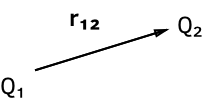
\includegraphics{skizzen/14/14_2B0}

$$ \boxed{\vec{F_{12}} = f\cdot\frac{Q_1\cdot Q_2}{r^2_{12}}\cdot\frac{\vec{r_{12}}}{|\vec{r_{12}}|} = f\cdot\frac{Q_1\cdot Q_2}{r^2_{12}}\cdot \hat{r}_{12}} $$

\noindent F ist definiert durch die Definition der Ladungseinheit:
\\
Internationales Messsystem (SI): $f=\frac{1}{4\pi\epsilon_0}$
\\
$\epsilon_0=8,854\cdot10^{-12}\frac{(As)^2}{Nm^2}$
\\
ist Dielektrizit\"{a}tskonste des Vakuums oder elektrische Feldkonstante
\\
$Q_1\cdot Q_2 > 0:$ Abstoßung
\\
$Q_1\cdot Q_2 < 0:$ Anziehung
\\
\subparagraph{Coulomb-Kraft}

\hfill\\

\boxed{\vec{F}_{12} = \frac{1}{4\pi\epsilon_0}\cdot\frac{Q_1\cdot Q_2}{r^2_{12}}\cdot\hat{r}_{12}}

\hfill\\

\noindent\fbox{%
\parbox{\textwidth}{%
	1 Coulomb ist diejenige elektrische Ladung, die eine gleich große Ladung im Abstand von 1m mit der Kraft von $8,9874\cdot10^9N$ abstößt	
}%
}

\subparagraph{Analogie Gravitation:} $\vec{F} = -\gamma\frac{m_1\cdot m_2}{r^2}\cdot\hat r$\\

Vergleiche Gravitation und Coulombkraft zwischen Elektron und Proton:

$$ |\vec{F}_C| = \frac{1}{4\pi\epsilon_0}\cdot\frac{|q_p|\cdot|q_e|}{r^2}= 2,3\cdot10^{ -28 } \frac{N}{r[m]^2} $$
$$ |\vec{F}_G|= \gamma\cdot m_e\cdot m_p  = 9,71\cdot10^{-68} \frac{N}{r[m]^2}$$

$$ \implies \frac{|F_G|}{|F_C|} = 4,2\cdot10^{-40} $$

\subparagraph{Wechselwirkung zwischen mehreren Ladungen}

\hfill\\

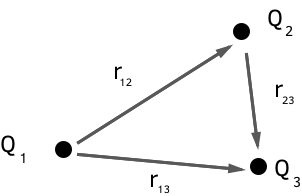
\includegraphics{skizzen/14/14_2B1}

\hfill\\

Die einzelnen Kräfte überlagern sich ungestört, (ungestörte Superposition)!\\

Kraft auf $$ Q_3: \vec{F}_3 = \bigg[\frac{Q_1\cdot Q_3}{r^2_{13}}\cdot\hat{r}_{13}+\frac{Q_2\cdot Q_3}{r^2_{23}}\cdot\hat{r}_{23}\bigg]$$ 


\subsection{Potenzielle Energie einer Ladungsverteilung}


\begin{align*}
\displaystyle W_{12} &= -\frac{1}{4\pi\epsilon_0}\cdot\int_{\infty}^{r} \frac{Q_1\cdot Q_2}{V^2}  \mathrm{d}V\\
&=\frac{1}{4\pi\epsilon_0} \big[\frac{Q_1\cdot Q_2}{V}\big]^{12}_\infty = \frac{1}{4\pi\epsilon_0}\cdot \frac{Q_1\cdot Q_2}{V_{12}}\\
W_{1,2,3} &= \frac{1}{4\pi\epsilon_0}(\frac{Q_1\cdot Q_3}{r_{13}}+\frac{Q_1\cdot Q_2}{r_{12}}+\frac{Q_2\cdot Q_3}{r_{23}})
\end{align*}\\

Anzahl an Summanden = Anzahl an Paaren\\

$\boxed{W = \bigg[\frac{1}{2}\sum_{i=1}^{N} \sum_{j≠i=1}^{N} \frac{Q_i\cdot Q_j}{r_{ij}}\bigg]\cdot \frac{1}{4\pi\epsilon_0}}\\$
\\
$\implies$ Aufsummieren auch unendlicher Ensembles möglich, wenn die Reihe konvergiert. 

\paragraph{Betrachte Kraft auf Probeladung in homogen geladener Kugel}

\hfill\\

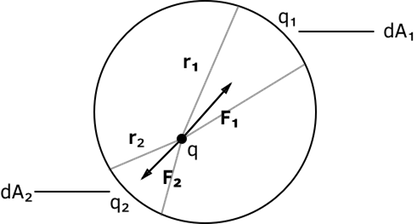
\includegraphics{skizzen/14/14_3B0}

\hfill\\

Für beliebe Räumlichelemente (und damit auch Flächenelemente) gilt:

$q_1 \propto \mathrm{d}A_1 \propto r_1^2$

$q_1 \propto \mathrm{d}A_1 \propto r_1^2$

Geometrie $\implies \frac{q_1}{q_2} = \frac{r_1^2}{r_2^2}$

Annahme: Kraft $\propto \frac{1}{r^n}$\\

\begin{align*}
	\vert\vec{F}_1\vert &= \frac{1}{4\pi\epsilon_0}\cdot\frac{q\cdot q_1}{r_1^n}\\
	\vert\vec{F}_2\vert &= \frac{1}{4\pi\epsilon_0}\cdot\frac{q\cdot q_2}{r_2^n}
\end{align*}\\

Geometrie einsetzen: 

$\frac{|\vec{F}_1|}{|\vec{F}_2|} = \frac{q_1}{r_1^n}\cdot \frac{r_2^n}{q_2} \overset{!}{=} 1 \implies n = 2$

Gesamtkraft verschwindet nur wenn $|\vec{F}| \propto \frac{1}{r^2}$

\subsection{Erzeugung el. Felder durch Ladungen}

	\subsubsection{Feld einer Punktladung:}
	
	\begin{align*}
		\vec{F} &= \frac{1}{4\pi\epsilon_0} \cdot \frac{q_1 q_2}{ |\vec{r}_{12}|^2 } \cdot \hat{r_{12}} \\
					&=q_1 \underbrace{ \cdot \frac{1}{4\pi\epsilon_0} \cdot \frac{q_2}{ |\vec{r}_{12}|^2 } \cdot \hat{r_{12}}  }_{\text{Feld von }q_2} \\
					&=q_1 \vec{E}(\vec{r})
	\end{align*}
	\begin{itemize}
		\item Felder einer Punktladung sind Zentralfelder mit Kugelsymmetrie
		\item Konvention: Feldlinien führen von positiver zu negativer Ladung
	\end{itemize}
	\begin{center}
		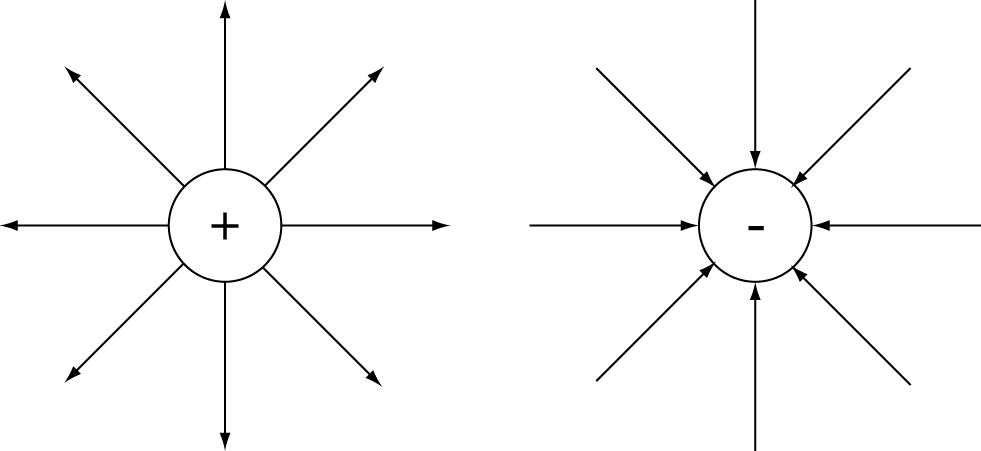
\includegraphics[width=0.7\linewidth]{skizzen/14/14_4B0}
	\end{center}

	$ \Rightarrow $ \underline{Punktladungsfelder sind inhomogen!}
	
	\subsubsection{Feld einer Verteilung von Punktladungen}
	N Ladungen bei $ \vec{r_i} $ 
	$$ \vec{E_i}(\vec{r}) = \frac{1}{4\pi\epsilon_0} \cdot \frac{q_i}{ | \vec{r} - \vec{r_i} |^2 } \cdot \frac{ \vec{r} - \vec{r_i}  }{ | \vec{r} - \vec{r_i}| }  $$
	Ungestörte Superposition:
	$$  \vec{E}(\vec{r}) = \frac{1}{4\pi\epsilon_0} \cdot {\displaystyle \sum_{i=1}^{N} \frac{q_i}{ | \vec{r} - \vec{r_i} |^2 } } \cdot \frac{ \vec{r} - \vec{r_i}  }{ | \vec{r} - \vec{r_i}| } $$
	\begin{minipage}{\textwidth}
		
		2 Ladungen, q ; -q : Feld eines Dipols 
		\begin{center}
			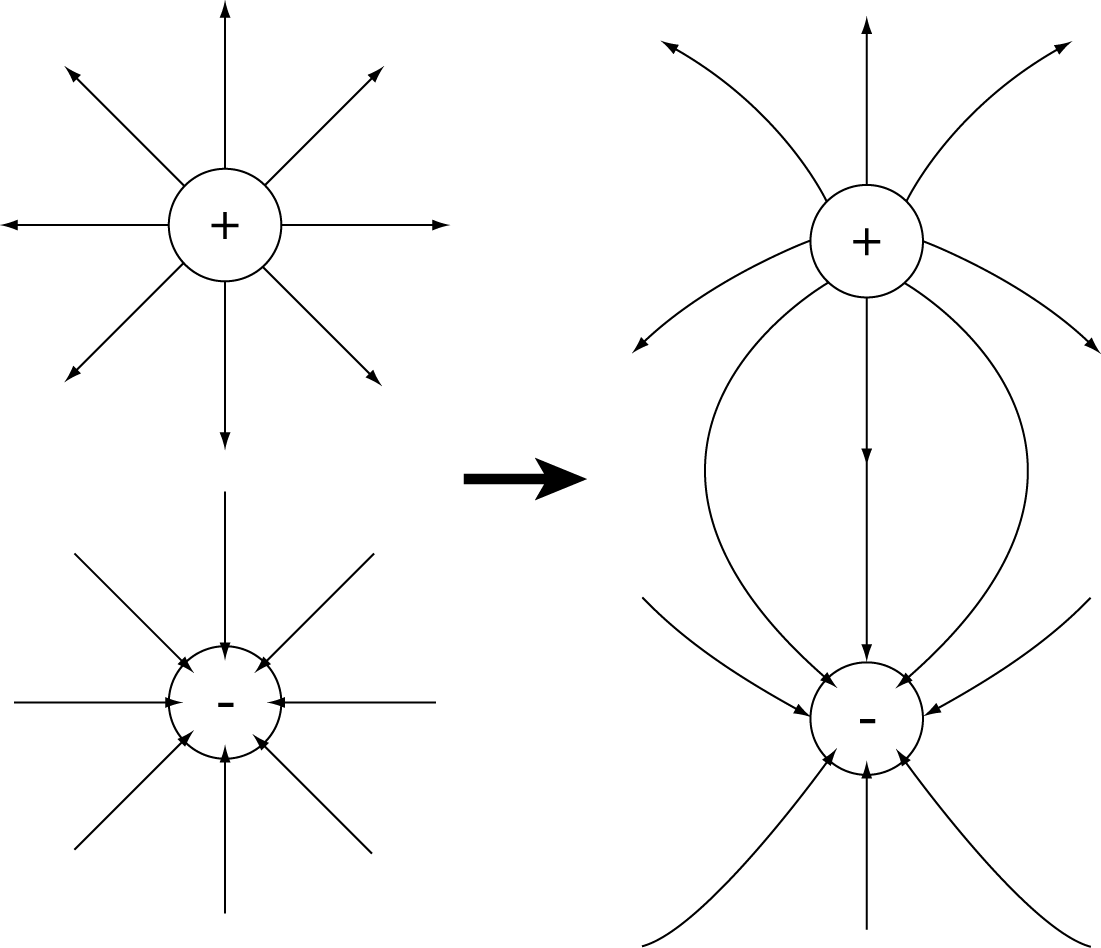
\includegraphics[width=0.4\linewidth]{skizzen/14/14_4B1}
		\end{center}
	
		2 Ladungen: q ; q 
		\begin{center}
			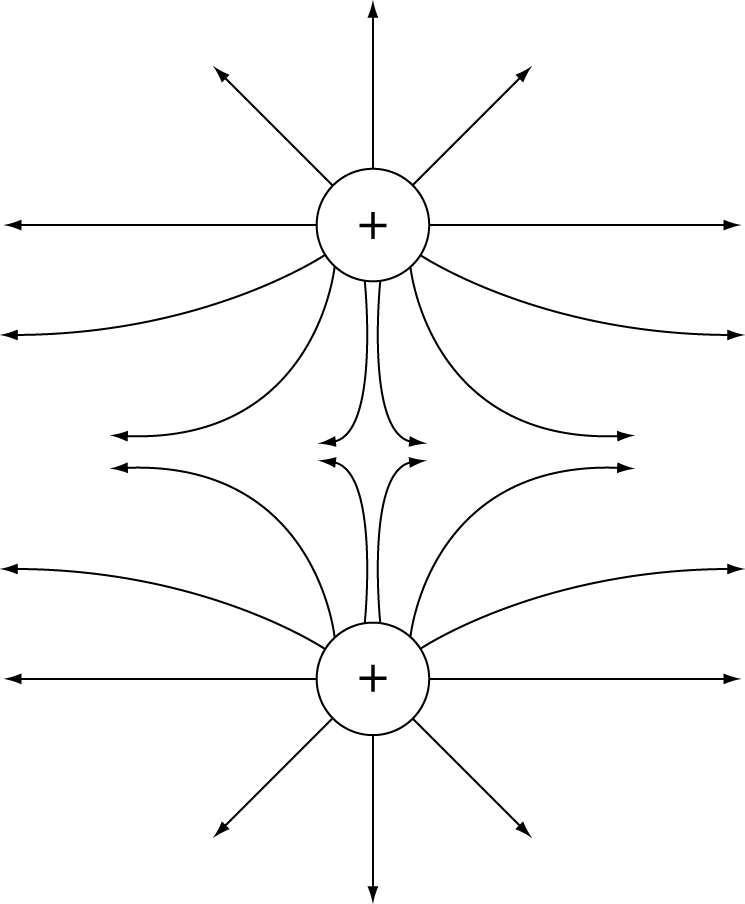
\includegraphics[width=0.4\linewidth]{skizzen/14/14_4B2}
		\end{center}
	
	\end{minipage}
	
	\begin{minipage}{\textwidth}
	
		Beispiele für "natürliche Dipole": \\
		\begin{enumerate}
			\item Neutrales Atom im homogenen $ \vec{E} $-Feld  
			\begin{center}
				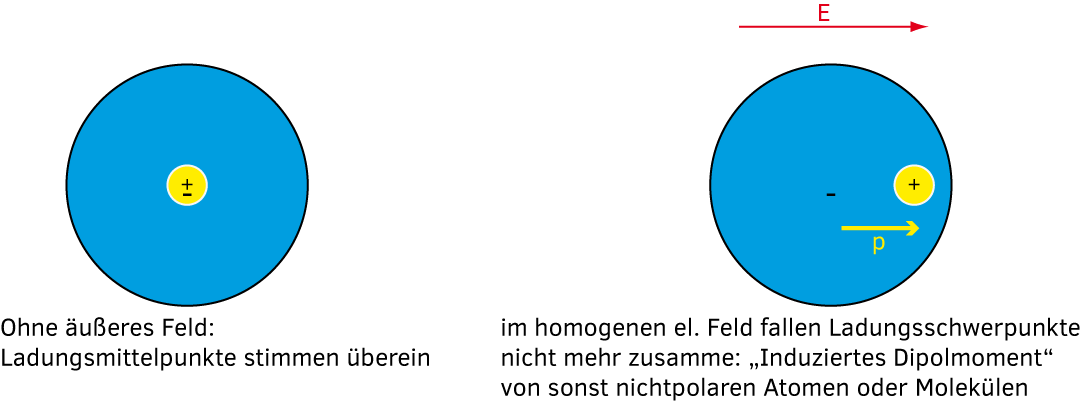
\includegraphics[width=0.9\linewidth]{skizzen/14/14_4B3}
			\end{center}
	
			\item Polare Molekühle mit permanentem Dipolmoment
			\begin{center}
				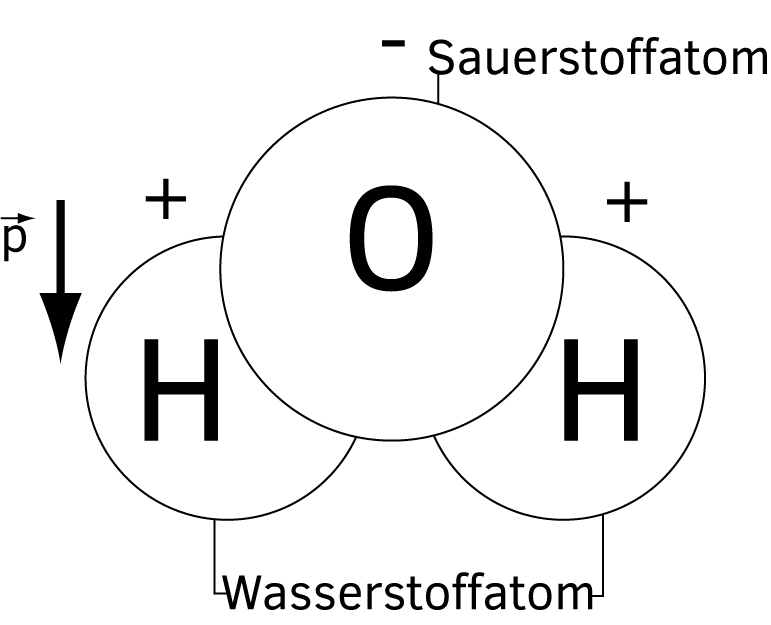
\includegraphics[width=0.4\linewidth]{skizzen/14/14_4B4}
			\end{center}
		
		\end{enumerate}
	
	\end{minipage}
	
	\subsubsection{Leiter im el. Feld und Influenz}
	Leiter: Ladungen sind \underline{frei} beweglich  \\
	Isolator: Ladungen sind ortsfest
	\begin{enumerate}
		\item $ \vec{E} = 0 $ im Inneren des Leiters 
		\begin{center}
			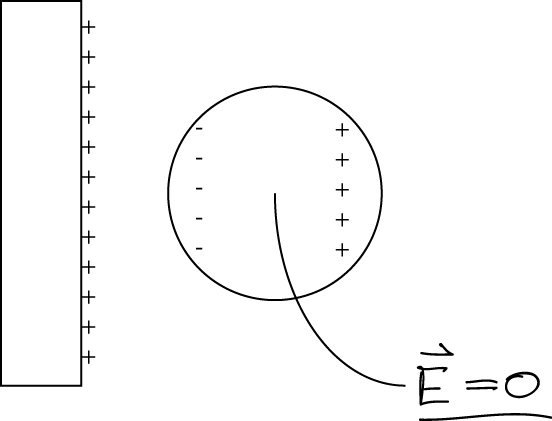
\includegraphics[width=0.4\linewidth]{skizzen/14/14_4B6}
		\end{center} 
		falls $ \vec{E} \neq 0 $: $ \vec{F} = q\vec{E} $ verschiebt Ladung bis $ \vec{E} = 0 $ ! 
		\item Es folgt, sich bei einem Leiter die (Netto-)Ladungen \underline{immer} an der Oberfläche befinden $ \Rightarrow $ Flächenladungsdichte $ \boxed{\sigma = \frac{dQ}{dA}} $
		\item $ \vec{E} $ immer $ \perp $ auf Leiteroberfläche
		\begin{center}
			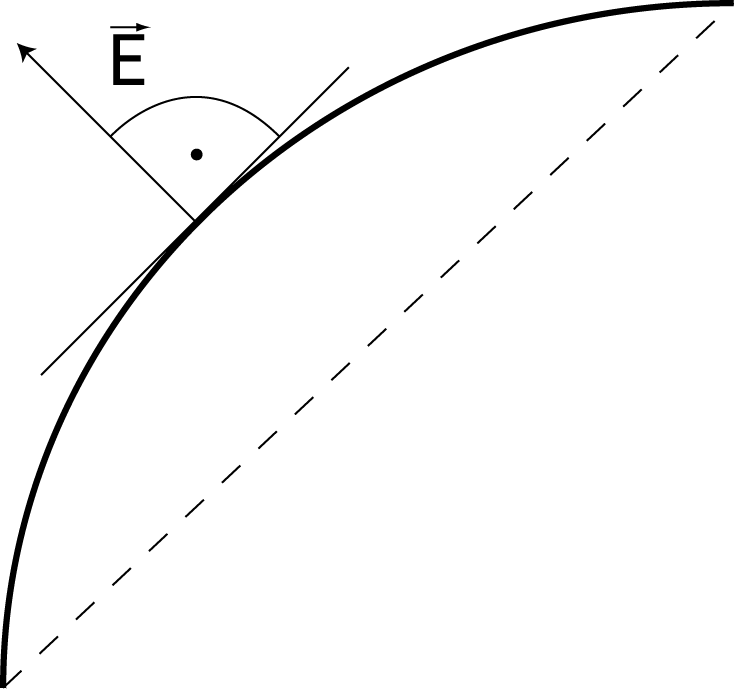
\includegraphics[width=0.4\linewidth]{skizzen/14/14_4B7}
		\end{center}
		(falls $ \vec{E}_{\shortparallel} \neq 0 $: Verschiebung der Ladung bis $ \vec{E}_{\shortparallel} = 0 $ !)

	\end{enumerate}
	\paragraph{\underline{Influenz}:} Räumliche Ladungstrennung in el. Leitern durch äu\ss{}eres $ \vec{E} $-Feld (Kontaktlos!), so dass das Innere des Leiters Feldfrei ist! 
	

		
	\subsection{Kontinuierliche Ladungsverteilung}
	
		Betrachte Ladungsverteilung über endliches Volumen $ V = {\displaystyle \int_V dV} $
		\begin{center}
			\hypertarget{ref1}{}
			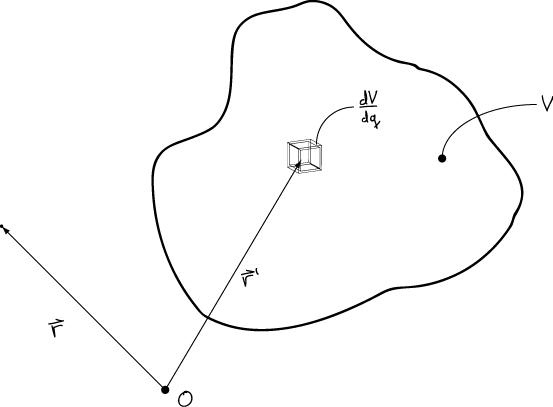
\includegraphics[width=0.5\linewidth]{skizzen/14/14_5B0}
			(\textasteriskcentered)
		\end{center}
		Ladungsdichte: $ \rho(\vec{r}) = \frac{dq(\vec{r})}{dV} $ \\
		Gesamtladung: $ Q = {\displaystyle\int_V dq} = {\displaystyle\int_V} \rho(\vec{r}) dV  $ \\
		Flächenladungsdichte: $ \sigma = \frac{dq}{dA} $ \\
		
		Integral über geschlossene Oberfläche: $ A = {\displaystyle\oint_A} dA $ \\
		1-dim Ladungsdichte: $ \lambda = \frac{dq}{dl} $ \\
		Länge $ l = {\displaystyle\int_l dl'} $ \\
		für \hyperlink{ref1}{(\textasteriskcentered)} :
		\begin{align*}
		d\vec{E}(\vec{r}) &= \frac{dq}{| \vec{r}-\vec{r}' |^3} \cdot (\vec{r}-\vec{r}') \cdot \frac{1}{4\pi\epsilon_0} \\
		\vec{E}(\vec{r}) &= \frac{1}{4\pi\epsilon_0} {\displaystyle\int_V dV} \left\{ \frac{dq}{dV} \cdot \frac{(\vec{r}-\vec{r}')}{| \vec{r}-\vec{r}' |^3} \right\} \\
		&=\underline{\frac{1}{4\pi\epsilon_0} {\displaystyle\int_V dV} \left\{ \frac{ \rho(\vec{r}) }{| \vec{r}-\vec{r}' |^3} \cdot (\vec{r}-\vec{r}') \right\}}
		\end{align*}
		
		\paragraph{Beispiel:} unendlich langer geladener Draht \\
		\begin{center}
			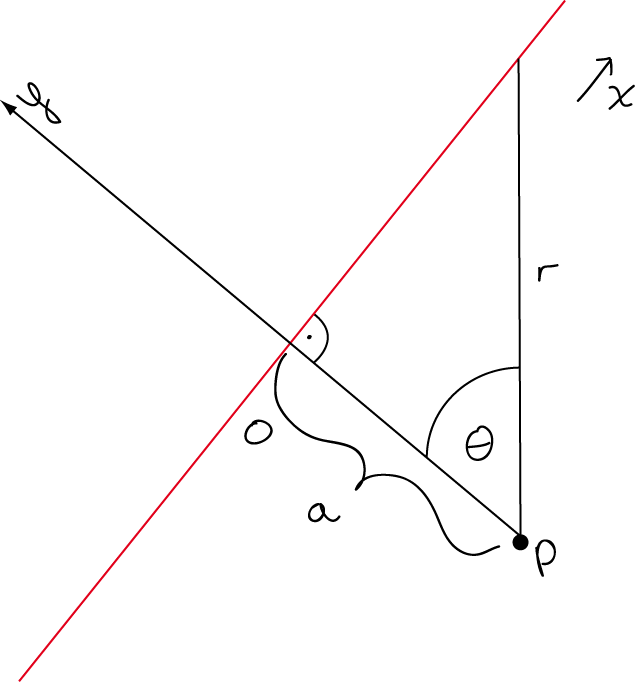
\includegraphics[width=0.5\linewidth]{skizzen/14/14_5B1}
		\end{center}
		\begin{align*}
		\frac{dq}{dx} = \lambda \text{ (lin. Ladungsdichte) } \\
		\text{Symmetrie: } E_x = E_z = 0 \\
		E_y = E \cdot \cos(\theta) \\
		dE_y& = | d\vec{E} | \cdot \cos (\theta) \\
		dE_y &= \frac{1}{4\pi\epsilon_0} \cdot 2 \cdot \frac{\lambda \cdot dx}{r^2 (\theta)} \cdot \cos (\theta) \hspace{1cm} ; \cos (\theta) = \frac{a}{r}&& \\
		&= \frac{1}{2\pi\epsilon_0} \cdot \lambda \cdot dx  \cdot \underline{\cos^2\theta} \cdot \cos\theta \\
		\hfill \\
		\tan\theta = \frac{x}{a} \Rightarrow \frac{dx}{d\theta} = \frac{a}{\cos^2\theta} \hspace{1cm} \Rightarrow dx = \underline{\frac{a}{\cos^2\theta} d\theta}
		\end{align*}
		
		\begin{align*}
		\Rightarrow dE_y &= \frac{1}{2\pi\epsilon_0} \cdot \lambda \cdot \frac{\cos\theta}{a} \cdot d\theta \\
		E_y &= \frac{1}{2\pi\epsilon_0} \cdot \frac{\lambda}{a} \cdot { \displaystyle\int_{0}^{\pi/2} \cos\theta d\theta } = \underline{\underline{\frac{1}{2\pi\epsilon_0} \cdot  \frac{\lambda}{a} }}
		\end{align*}

		
	
\subsection{Elektrischer Fluss und Satz von Gauß}

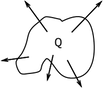
\includegraphics{skizzen/14/14_6B0}
		
Zusammenhang zwischen "Elektrischem Fluss" (Feldliniendurchsatz) durch eine Oberfläche und der eingeschlossenen Ladung.

$\implies$ Allgemeinere Formulierung des Coulomb-Gesetzes

\subsubsection{Definition: Fluss $\phi$ eines Vektorfeldes $\vec{E}$ durch einen Fläche A:}

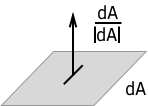
\includegraphics{skizzen/14/14_6B1}


$\phi= \int_A \vec{E}\cdot d\vec{A}$

\begin{align*}
	d\vec{A}:&\text{Richtung }\perp \text{ Fläche (nach Außen)}\\
	&\text{Richtung der Flächennormale}
\end{align*}\\

Betrag dA: Größe der Fläche

\subparagraph{Spezialfälle}\\

$\vec{E}-homogen$
$\vec{E}\cdot d\vec{A}= E\cdot dA\cdot \cos\alpha$

\begin{itemize}
	\item $\alpha=0°: \vec{E}\parallel d\vec{A}: \vec{E}\cdot d\vec{A}=E\cdot dA$\\
	\item $\alpha=90°: \vec{E}\perp d\vec{A}: \vec{E}\cdot d\vec{A}=0$
\end{itemize}

\subsubsection{Gauß'scher Satz}

$\boxed{\displaystyle\phi=\oint_{\underset{geschlossen}{A}}\vec{E}\cdot d\vec{A}=\frac{Q_{eingeschlossen}}{\epsilon_0}}$\\

Der elektrische Fluss durch einer belieben geschlossenen Oberfläche hängt weder von der Form der Oberfläche, noch von der Ladungsverteilung $\varrho(\vec{r})$ ab, sondern nur von der eingeschlossenen Gesamtladung Q.\\

\subparagraph{Mathematisch gilt:}

\begin{align*}
	\oint_{A}\vec{E}\cdot d\vec{A}&=\int_{V} div\cdot \vec{E}\cdot dV\\
	&=\int_{V}\vec{\nabla}\cdot\vec{E}\cdot dV
\end{align*}

\begin{align*}
	\implies \int_{V}\vec{\nabla}\vec{E}dV & =\frac{1}{\epsilon_0}\int_{V}\varrho(\vec{r})dV\\
	&=\vec{\nabla}\vec{E}=\frac{\varrho(\vec{r})}{\epsilon_0}
\end{align*}

Die Ladungsverteilung im Raum ist die lokale Quelle ($\varrho(\vec{r})>0$) bzw. Senke ($\varrho(\vec{r})<0$) des elektrischen Feldes.

\subsubsection{Beispiele}

(i)Feld einer Punktladung\\

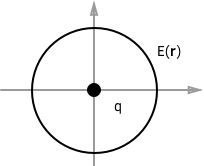
\includegraphics{skizzen/14/14_6B2}\\

\begin{itemize}
	\item Geeignete Wahl von A: Kugeloberfläche
	\item Symmetrie: $\vec{E}(\vec{r})=E(r)\cdot\hat e_r$
	\item $\implies \vec{E}\parallel d\vec{A}$
\end{itemize}

\begin{align*}
	\phi=\oint_{A}\vec{E}(\vec{r})\cdot\mathrm{d}\vec{A} & = \oint_{A}E(r)\cdot\hat{e}_r\cdot\mathrm{d}\vec{A}\\
	&=\oint_{A}E(r)\cdot\mathrm{dA}\\
	&= E(r)\cdot\oint_{A}\mathrm{dA}\\
	&= E(r)\cdot4\pi r^2
\end{align*}

Gauß: $\phi\overset{!}{=} \frac{Q}{\epsilon_0}=E(r)\cdot4\pi r^2 \implies \underline{E(r)=\frac{1}{4\pi\epsilon_0}\cdot\frac{Q}{r^2}}$\\

(ii) Ladung auf beliebig geformten \underline{Leitern}\\

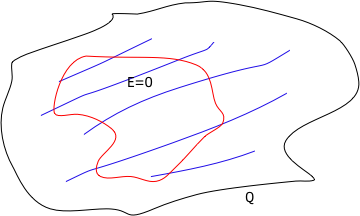
\includegraphics{skizzen/14/14_6B3}\\

$\phi=\oint_{A}\vec{E}d\vec{A}=\frac{Q}{\epsilon_0}=0$\\

(iii) Feld einer \underline{leitenden} Kugel mit Ladung Q: (Ladung auf der Oberfläche)\\

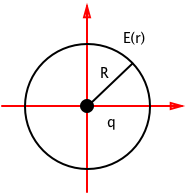
\includegraphics{skizzen/14/14_6B4}\\

$ \vec{E}(\vec{r})= E(\vec{r})\cdot\hat{e}_r $

$ r<R: E=0 $

$ r>R: \phi=\oint_{A}E(r)\mathrm{dA}=E(r)\cdot4\pi r^2 $

$ \phi=\frac{Q}{\epsilon_0} $

$ \implies \underline{E(r)= \frac{1}{4\pi\epsilon_0}\cdot\frac{Q}{r^2}} $

\hfill\\

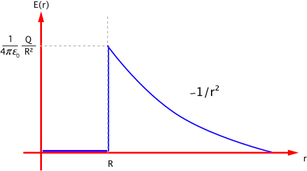
\includegraphics{skizzen/14/14_6B5}\\

(iv) Feld einer homogen geladenen Kugel\\

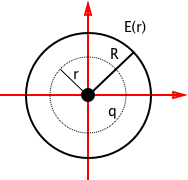
\includegraphics{skizzen/14/14_6B6}\\

$ \rho =\frac{Q}{\frac{4}{3}\pi R^3} \text{ für }r<R $
$ \rho=0 \text{ für }r>R$

\underline{$r<R$}:

$ \phi=\oint_{A}\vec{E}\cdot\mathrm{d}\vec{A} = E(r)\cdot4\pi r^2=\frac{Q_{in}}{\epsilon_0}$

$ Q_{in} = Q\cdot\frac{r^3}{R^3} $

\hfill\\

$\boxed{ \implies E(r)=\frac{1}{4\pi\epsilon_0}\cdot\frac{Q}{R^3}\cdot r }$

\hfill\\

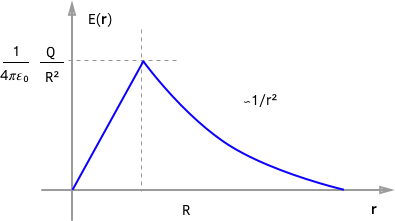
\includegraphics{skizzen/14/14_6B7}\\

$\implies$ Von Außen ist nicht feststellbar, ob die geladene Kugel massiv oder hohl ist (Leiter oder homogen geladener Isolator)!\\

(v) Unendlich lnager homogen geladener Draht\\

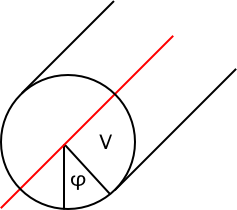
\includegraphics{skizzen/14/14_6B8}\\

Zylinderkoordinaten:\\

$ \lambda=\frac{dq}{dL}=(\frac{Q}{R})\leftarrow $ als endliche lange l

$ \vec{E}(\vec{r})=\vec{E}(r)=E(r)\cdot\hat{e}_r $

$ \phi=\oint_{A}\vec{E}\cdot d\vec{A}=\oint_{A}E(r)dA=E(r)\oint_{A}da= E(r)\cdot 2\pi r l $

$ \phi=\frac{Q_{ges}}{\epsilon_0}\implies E(r)= \frac{Q_{ges}}{2\pi\epsilon_0\cdot rl} $

$ E(r)= \underline{ \frac{\lambda}{2\pi\epsilon_0}\cdot\frac{1}{r}}$\\

(vi) Unendlich langer, homogen geladener leitender Zylinder\\

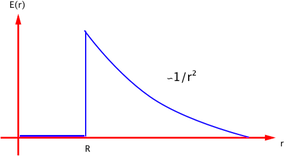
\includegraphics{skizzen/14/14_6B9}\\

(vii) Feld einer homogen geladener unendliche leitenden Ebene\\

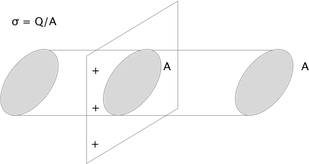
\includegraphics{skizzen/14/14_6BA}

\hfill\\

$ \sigma=\frac{Q}{A} $

$ \displaystyle\phi = \oint_{A}\vec{E}\cdot d\vec{A}=\int_{A, stirn}^{} \vec{E}\cdot d\vec{A}+\int_{A, mantel}^{} \vec{E}\cdot d\vec{A}   $

$ \vec{E} $-Ebene

$ \implies $ Beitrag Über Mantelfläche verschwindet $ (d\vec{A}\perp\vec{E}) $

$ \phi=\oint_{A} \vec{E}d\vec{A}=2\cdot E\cdot A_{stirn}\overset{G.S.}{=}\frac{Q}{\epsilon_0}$ 

$ \underline{\implies E=\frac{\sigma}{2\epsilon_0}} $

\subsection{Das elektrische Potenzial}\\

Coulombkraft: Zentralkraft, konservativ\\
$\implies \exists$ potentielle Energie (siehe 14.3)\\
für Ladungen $q_0$ im $\vec{E}$-Feld gilt:\\

\hfill\\
$\boxed{\displaystyle E_{pot}(\vec{r})=-q_0\cdot\int_{\infty}^{\vec{r}} \vec{E}(\vec{r})\cdot d\vec{r}}$
\hfill\\

Für das elektrische Potenzial $ \varrho(\vec{r}) $ gilt:

\hfill\\
$\boxed{\displaystyle\varphi=-\int_{\infty}^{\vec{r}} \vec{E}(\vec{r})\cdot d\vec{r} = \frac{1}{q_0}E_{pot}\cdot (\vec{r})}$
\hfill\\

$\rightarrow$ Beachte: Arbeit ist unabhängig vom Weg!\\
Verschiebe $q_0$ von $\vec{r}_1$ nach $\vec{r}_2$; die benötigte Arbeit ist:\\

\begin{align*}
	\displaystyle W_{12}= \int_{\vec{r}_1}^{\vec{r}_2} \vec{F}(\vec{r})\cdot d\vec{r} & = q_0\int_{\vec{r}_1}^{\vec{r}_2} \vec{E}(\vec{r})\cdot d\vec{r} \\
	&\underline{ =q_0\cdot(\varphi(\vec{r}_1)-\varphi(\vec{r}_2))}
\end{align*}

$ \varrho(\vec{r}) $ nur bis auf Integrationskonste bestimmt!\\
Die Potentialdifferenz zwischen zwei Punkten:\\

$ U = \varphi(\vec{r}_1)-\varphi(\vec{r}_2) = \frac{W_{12}}{q_0}$ heißt elektrische Spannung!\\

$q_0\cdot U$ ist die Arbeit, die man braucht um $q_0$ von $ \vec{r}_1 $ nach $ \vec{r}_2 $ zu bringen!\\

$[U]= 1Volt = 1V = 1\frac{I}{C}$\\

\paragraph{Beachte:} $ \varphi(\vec{r}_1)-\varphi(\vec{r}_2) = -\oint \vec{E}(\vec{r})\cdot d\vec{r}= 0!!$\\

Typische Spannungen:
\begin{align*}
	Batterie&$: 1,5V$\\
	Stadtnetz&$: 220V$\\
	Überlandleitung&$: 250kV$\\
	Blitz&$: 10-15MV$
\end{align*}

\subparagraph{Beispiele:}
\\
(i) Punktladung:

\begin{align*}
	\displaystyle \varphi(\vec{r})&= -\int \vec{E}(\vec{r'})\cdot d\vec{r'}; \vec{E}=E\cdot\hat{e}_r\\
	\displaystyle &=-\frac{q_1}{4\pi\epsilon_0}\cdot\int_{\infty}^{r} \frac{d\vec{r}}{r^2}
\end{align*}

$\underline{\varphi(\vec{r})=\varphi(r)=\frac{q_1}{4\pi\epsilon_0\cdot r}}$\\

\subparagraph{Äquipotenzialflächen:} r=const.\\
(in 3D: Kugelflächen\\
in 2D: Kreise)

\hfill\\

(ii) Mehrere Punktladungen\\

$\displaystyle\varphi(\vec{r})=\frac{1}{4\pi\epsilon_0}\cdot\sum_{i} \frac{q_i}{|\vec{r}-\tilde{\vec{r}}_i|}$

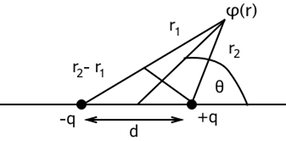
\includegraphics{skizzen/14/14_7B0}

$ \varphi(\vec{r})=\frac{1}{4\pi\epsilon_0}\cdot(\frac{q}{r_1}-\frac{q}{r_2})=\frac{q}{4\pi\epsilon_0}-\frac{r_2-r_1}{r_1\cdot r_2} $

\begin{align*}
	\text{für } \underbrace{d\ll r}_{\text{Fernfeld}}:& r_1\cdot r_2 = r^2\\
	&r_2-r_1=d\cdot\cos\theta
\end{align*}

$ \varphi(\vec{r})=\varphi(r)=\frac{q\cdot d\cdot \cos\theta}{4\pi\epsilon_0\cdot r^2} = \frac{\varphi\cdot\cos\theta}{4\pi\epsilon_0}\cdot\frac{1}{r^2} $

\subparagraph{Potenzialverteilung:}
\hfill\\
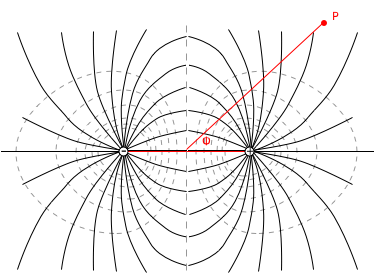
\includegraphics{skizzen/14/14_7B1}
\\
(iii) Kontinuierliche Ladungsverteilung:\\

$ \displaystyle\varphi(\vec{r})=\frac{1}{4\pi\epsilon_0}\cdot\int_{\tilde{V}} \frac{dQ}{|\vec{r}-\tilde{\vec{r}}|} = \frac{1}{4\pi\epsilon_0}\cdot\int_{\tilde{V}} d\tilde{V}\bigg\{\frac{\varphi(\vec{r})}{|\vec{r}-\tilde{\vec{r}}|}\bigg\}$\\

\subsubsection{Elektrisches Feld und Potenzial}

$ \varphi(\vec{r}): $ Skalare Größe, manchmal einfache zu berechen als $ \vec{E}(\vec{r}) $\\

$\implies \vec{E}(\vec{r}) $ aus $ \varphi(\vec{r}) $ bestimmen?\\

\begin{align*}
	\varphi=\varphi(\vec{r}) &= \varphi(x,y,z); \vec{E}= \vec{E}(\vec{r})=\begin{pmatrix}E_x\\ E_y\\ E_z\end{pmatrix}\\
	d\vec{r}&= \begin{pmatrix}dx\\ dy\\ dz\end{pmatrix}
\end{align*}

\underbrace{d\varphi}_{\text{vollständiges Differential}}= -\vec{E}d\vec{r} = - (E_xdx+E_ydy+E_zdz)(*)\\

d\varphi=\frac{\partial\varphi}{\partial x}\cdot dx +\frac{\partial\varphi}{\partial y}\cdot dy+\frac{\partial\varphi}{\partial z}\cdot dz (**)\\

(*),(**):  \left.\begin{aligned} E_x= -\frac{\partial\varphi}{\partial x}\\ E_x= -\frac{\partial\varphi}{\partial x}\\ E_x= -\frac{\partial\varphi}{\partial x} \end{aligned}\right\} \implies \underline{\vec{E}=-grad\varphi}\\

$\vec{E}$ zeigt in Richtung des betragsmäßig größten Anstiegs von $\varphi$, allerdiings in abnehmende Richtung.\\

Äquipontenziallinie: $ d\varphi= -\vec{E}\cdot d\vec{r} $\\
längst einer solchen Linie ist: $ d\varphi=0\implies -\vec{E}\cdot d\vec{r}=0 $\\
$ \implies \underline{\vec{E}\perp d\vec{r}} $\\


\subparagraph{Beispiel:} Punktladung\\

$ \varphi(\vec{r})=\frac{q}{4\pi\epsilon_0}\cdot \frac{1}{r} $\\

Kugelkoordinaten, Kugelsymmetrie: $ \vec{E}=-\nabla\cdot\varphi=-\frac{\partial\varphi}{\partial r}\cdot \hat{e}_r $\\

$ \frac{\partial\varphi}{\partial r}=-\frac{q}{4\pi\epsilon_0}\cdot\frac{1}{r^2} \implies \vec{E}=\frac{q}{4\pi\epsilon_0}\cdot \frac{1}{r^2}\cdot\hat{e}_r$\\

\subsubsection{Poisson- und Laplace Gleichung:}\\

Gauß'scher Satz: $div\vec{E}=\vec{\nabla}=\frac{\varrho}{\epsilon_0}$\\
Potenzial: $\vec{E}=-\vec{\nabla}\varphi$\\

Einsetzen: $\boxed{div grad \varphi=\underbrace{\vec{\nabla}\cdot\vec{\nabla}}_{\Delta}\cdot\varphi = -\frac{\varrho}{\epsilon_0}}$\\

$ \Delta\varphi=\big(\frac{\partial^2}{\partial x^2}+\frac{\partial^2}{\partial y^2}+\frac{\partial^2}{\partial z^2}\big)\cdot\varphi $\\

\subparagraph{Spezialfall:}\\

\varphi=0
\implies \text{Laplace-Gleich}= \underline{\Delta\varphi=0}

\hfill\\

\subsection{Elektrisches Feld in der Umgebung von Leitern}\\

Gauß'scher Satz: $ \oint_{A}\vec{E}\cdot d\vec{A}=0 \implies \varrho=0 $\\
(Leiter im Inneren Feldfrei!)\\

Potenzial: $\varphi(r)=-\int\vec{E}d\vec{r}= \text{const.}$\\

$\implies$ \underline{Leiteroberfläche ist Äquipotenzialfläche}\\

\paragraph{Beispiel: Elektrisches Feld an Kugeloberfläche:}
\hfill\\
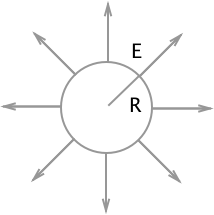
\includegraphics{skizzen/14/14_8B0}\\

$$ E_\perp $$ für jede Leiteroberfläche berechenbar:\\

$ \displaystyle\oint_{A}\vec{E}\cdot d\vec{A} = \frac{Q}{\epsilon_0} $\\

\paragraph{Beispiel:}
\hfill\\
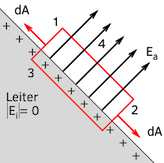
\includegraphics{skizzen/14/14_8B1}
\\
\subparagraph{Fläche:}
\hfill\\
1,2: \vec{E}\perp d\vec{A} \implies "0"\\
3: \vec{E}=0 \implies 0\\
4: E\cdot A= \frac{Q}{\epsilon_0}\\
\hfill\\

$ \implies \vert\vec{E}\vert = \frac{1}{\epsilon_0}\cdot \frac{Q}{A} = \frac{1}{\epsilon_0}\cdot\sigma $

$\implies$ Die Größe von $E_\perp$ an der Oberfläche ist $\frac{\sigma}{\epsilon_0}$!\\

\subparagraph{Weiter mit der Kugel:} $ E_a= \frac{\sigma}{\epsilon_0}=\frac{1}{\epsilon_0}\cdot\frac{Q}{4\pi\cdot R^2} $\\

$ \varphi = \frac{Q}{4\pi\epsilon_0\cdot R} \implies E_a=\frac{\varphi}{R}$\\

Bei gegebenen Potenzial ist Feldstärke an der Oberfläche umgekehrt proportional zum Kreis…radius!\\

Lokal: $ \vert\vec{E}\vert = \frac{\sigma}{\epsilon_0}=\frac{\varphi}{R} $\\

\underline{R Klein $\implies \varphi$ groß, $\sigma$ groß}\\

\subsubsection{Anwendungen:} Feldemmissions-Elektronenmikroskop:
\hfill\\
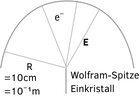
\includegraphics{skizzen/14/14_8B2}\\

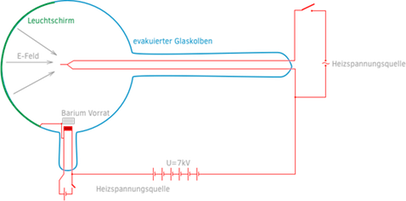
\includegraphics{skizzen/14/14_8B3}\\

$ \vert\vec{E}\vert = \frac{\varphi}{R}= \frac{10kV}{10^{-7}m} = 10^11\frac{V}{m} $ an der Wolfram-Spitze\\
Bewegung der Elektronen Entlang der Feldlinien\\
\begin{itemize}
	\item vergrößertes Bild der Wolfram-Spitze\\
	\item Vergrößerung: $\frac{R_{Schirm}}{R_{Spitze}}\approx \underline{10^6}$
	\item so erstmals Atome sichtbar gemacht
	\item Objekte $<10^{-9}m \implies <1mm!$
\end{itemize}

\subsubsection{Elektrisches Feld zwischen geladenen Leitern}

\paragraph{Anwendung:}2 isolierte, entgegengesetzt geladene Leiter, ($\implies$ Kondensator)
\hfill\\

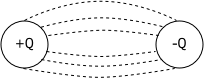
\includegraphics{skizzen/14/14_8B4}\\

Coulomb: $\vert\vec{E}\vert\propto\vert Q\vert$\\
Spannung: $ U_{21}=\varphi_2-\varphi_1 = -\displaystyle\int_{1}^{2} \vec{E}\cdot d\vec{r}\propto Q $ ist unabhängig vom Weg!\\

$ \implies Q\propto U $\\

Proportionalitätskonstante?

$\boxed{Q=C\cdot U}$\\

C:Kapazität\\
Einheit $[C]=\frac{1C}{1V}=1F$ (Farad)\\

\begin{align*}
	typisch:& 10^{-6}F=1\mu F\\
	& 10^{-9}F=1nF\\
	& 10^{-12}F=1pF
\end{align*}\\

\subsubsection{Berechnung der Kapazität:}
\hfill\\
Erinnerung: homogen geladene Platte: $E=\frac{\sigma}{2\epsilon_0}$\\

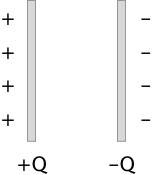
\includegraphics{skizzen/14/14_8B5}\\

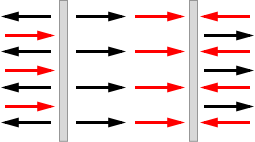
\includegraphics{skizzen/14/14_8B6}\\

Im Außenraum: Kompensation\\
Im Innenraum: Addition\\

Im Innenraum: $\vert\vec{E}\vert=\frac{\sigma}{\epsilon_0}$\\

\subsubsection{Feldstärke im Inneres eines Plattenkondensator:}

\hfill\\
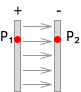
\includegraphics{skizzen/14/14_8B7}
\hfill\\

Seicherung von Ladungen auf voneinander isolierten leitenden Platten, Aufladung über Spannungsquelle oder Batterie.\\

Spannungspotenzialdifferenz: $ U_{21}=p_2-p_1=\int \vec{F}d\vec{r}=E\cdot d $\\
$ U = Ed=\frac{\sigma}{\epsilon_0}\cdot d = \frac{Q}{\epsilon_0\cdot A}\cdot d $\\
mit $Q=C\cdot U$ folgt $ \underline{C=\frac{\epsilon_0 A}{d}} $\\

$\boxed{\vert\vec{E}\vert=\frac{Q}{\epsilon_0\cdot A}}$ ist unabhängig von d\\

$\boxed{C=\epsilon_0\cdot \frac{A}{d}}$ ist eine rein geometrische Größe\\

$d\uparrow \implies C\downarrow \implies U\uparrow$\\

$d\downarrow \implies C\uparrow \implies U \downarrow$\\


\subsubsection{Realisierung von Kondensatoren:}\\

Großes C: A groß, d klein\\
Beidseitiges Bedampfte dünne Kunststofffläche, dann aufrollen, $\implies$ Kunststofffolienkondensator.\\

Größenordnung: $\begin{equation} \left. \begin{aligned} d=1mm\\ A=1cm^2\end{aligned}\right\}C=\epsilon_0\frac{A}{d}\end{equation}\\
	 \begin{align*}&=8,8\cdot 10^{-12}\frac{C^2}{Nm^2}\frac{10^{-4}m^2}{10^{-3}m}\\
	 &=0,9\cdot 10^{-12}F\\
	 &\approx \underline{1pF} \times \text{ Anzahl der Lagen}
	 \end{align*}$

\subsubsection{Energie eines aufgeladenen Kondensators}\\

Kondensator C sie mit Ladung q aufgeladen: $U=\frac{q}{c}$\\
Die Arbeit, die zum Aufbringen einer weiteren Ladung benötigt wird, hängt vom aktuellen Ladungszustand ab:\\

\begin{align*}
	dW&=dq\cdot U(q)\\
	&=dq\cdot\frac{q\cdot d}{A\cdot \epsilon_0}
\end{align*}\\

$W=\int_0^Q dW= \frac{d}{A\epsilon_0}\int_0^Q q/cdot d\cdot q= \frac{1}{2}\frac{1}{C}Q^2=\underline{\frac{1}{2}\cdot C\cdot U^2} $\\

Energiedichte: $ \underbrace{\frac{W}{V}}_{A\cdot d}=\frac{1}{2}\frac{\epsilon_0A}{d}\frac{1}{Ad}E^2d^2=\underline{\frac{1}{2}\epsilon_0E^2}$\\

(Dieses Ergebnis gilt auch für andere Feldverteilungen, nicht nur im Plattenkondensator)\\
$\rightarrow$ Feldenergie $\propto E^2$ (später wichtig!)\\

$\implies$ wichtige Anwendung: Schnelle Entladung eines langsam aufgeladenen Kondensators $\implies$ Kurzzeitig hohe Leistung!\\
\subparagraph{Beispiele}: Defibrilator, Blitzlicht…\\

\subsubsection{Entladen eines Kondensators}\\

$C=8\cdot 20\mu F; U=500V\\ W=\frac{1}{2}\cdot CU^2=\frac{1}{2}\cdot 16\cdot 10^{-5}F\cdot 25\cdot 10^4V^2\\ =\underline{20J}$\\
Entladung in \undertline{1ms} $\rightarrow$ \underline{20kW}\\

Defibrilator: $~ 100 - 800 kW$\\

\subparagraph{Fusionsanlage:}\\
Kondensatorbatteri ermöglichen W ~ $10^6$J\\
Entladung in 3ns\\
$\implies P = 3\cdot 10^{14}W$\\

\subsubsection{Kraft zwischen Zwei Kondensatorplatten}
\hfill\\
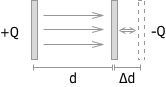
\includegraphics{skizzen/14/14_8B8}
\hfill\\
Anziehungskraft zwischen entgegengesetzt geladenen Kondensatorplatten\\
$\implies$ Arbeit gegen Kraft F, um Abstand um $\Delta d$ zu erhöhen.\\

Volumenänderung: \begin{align*}
	&\Delta V= A\cdot \Delta d\\
	&\Delta W= \frac{1}{2}\cdot \epsilon_0\vert\vec{E}\vert^2\cdot A\cdot \Delta d\\
	&\Delta W= F\cdot \Delta d \implies \underline{F}=\frac{\epsilon_0}{2}\cdot\vert\vec{E}\vert^2\cdot A=\underline{\frac{\epsilon_0}{2}\bigg(\frac{V}{d}\bigg)^2\cdot A\propto V^2}
\end{align*}\\

\subsubsection{Kraft zwischen Kondensatorplatten}\\

$U=2000V; d=10mm; ⌀=30cm \implies A=0,071m^2\\ F=\frac{\epsilon_0}{2}\bigg(\frac{V}{d}\bigg)^2\cdot A\=…=0,0197N$\\

Die äquivalente Masse wird von der Waage angezeigt:\\

$M=\frac{F}{g}=1m29g (\text{ gemessen}:m=1,33g)$\\

Verdopplung von U auf $4000V \implies 4-$Fache Masse. (gemessen: $m\approx 5,22g$)\\

\subsection{Isolatoren (Dielektrikum) im elektrischen Feld}














\end{document}
